% This version of CVPR template is provided by Ming-Ming Cheng.
% Please leave an issue if you found a bug:
% https://github.com/MCG-NKU/CVPR_Template.


%\documentclass[review]{cvpr}
\documentclass[final]{cvpr}

\usepackage{times}
\usepackage{epsfig}
\usepackage{graphicx}
\usepackage{amsmath}
\usepackage{amssymb}
\usepackage{subfigure}
%\usepackage{xcolor}
\usepackage{appendix}
%\usepackage[table,xcdraw]{xcolor}
% Include other packages here, before hyperref.

% If you comment hyperref and then uncomment it, you should delete
% egpaper.aux before re-running latex.  (Or just hit 'q' on the first latex
% run, let it finish, and you should be clear).
\usepackage[pagebackref=true,breaklinks=true,colorlinks,bookmarks=false]{hyperref}
\usepackage{listings}
\def\cvprPaperID{****} % *** Enter the CVPR Paper ID here
\def\confYear{CVPR 2021}
%\setcounter{page}{4321} % For final version only


\begin{document}

%%%%%%%%% TITLE
\title{How can we predict rental price from web data?}

\author{
% For a paper whose authors are all at the same institution,
% omit the following lines up until the closing ``}''.
% Additional authors and addresses can be added with ``\and'',
% just like the second author.
% To save space, use either the email address or home page, not both
Longtian Qiu\\
University of Shanghaitech\\
{\tt\small qiult@shanghaitech.edu.cn}
}

\maketitle


%%%%%%%%% ABSTRACT
\begin{abstract}
\textbf{With the rapid development of Internet industry, the real estate agency has been offering rental service by providing the information of apartments and houses for rent on the website. In this project, we propose a pipeline from collecting data to predicting the rental price for apartments and houses in shanghai. We crawl the room information at \textit{lianjia.com} by python script and generate feature vector for each room. We mainly explore two categories of algorithm to predict the rental price, neural networks and regression algorithm. Experiments on collected data set shows that given the size of the data set, the regression methods outperform the neural networks. The results are visualized as graphs and heat maps.}
\end{abstract}

%-------------------------------------------------------------------------
\section{Introduction}
Web crawlers are programs designed to collect the information from Internet. With the prosperity of the Internet, large amounts of data are available on various websites and social media, however, it's not feasible for researchers to collect these information by hands. The automatic scripts collecting data from internet are basic tools for data mining.

Feature generation is of primary importance in any regression or classification tasks, feature vector are used to represent the property of an object. Normally feature vector consist of numerical values which is called structured data. The main purpose of feature generation is to convert the unstructured raw data to structured feature vectors while keep as much as possible original information in the raw data.

Regression algorithms in machine learning are basically categorized into two class, linear and non-linear regression algorithm. The regression algorithms learn the relationship within the training data by finding the weight which leads to minimum loss value and predict a continuous numerical value given new data.

Neural network consist of multiple layers of nodes, where nodes are connected by edges with weights. The neural network learn the relationship within the data by optimizing the weights in the edges during the iteration of forward propagation and backward propagation. Compare with the regression algorithms, neural networks are able to learn more complex relationships within data given a sufficient size of data, however, the regression algorithms may perform a relative good result given a small data set.

\section{Data Collection}
\subsection{Methodology}
The \textit{linajia.com} website is a relatively simple one from the perspective of web developer. There is no anti-scraping technology such as encrypted html code or authentication restriction. Most information can be extracted by parsing the page html code with the help of beautiful soup 4, a python library for parsing html code. The information of recommending house and nearby house are passed by a request \textit{https://sh.lianjia.com/zufang/aj/house/similarRecommend} and we make an extra request to get the data.
There are many crawl scripts for collecting the rental house in \textit{linajia.com} available on github, however they are not designed to fetch complete information of house for rent, usually only the summary and price of the house are collected. We build crawler on the template of \textit{https://github.com/jumper2014/lianjia-beike-spider} and fetch the information in the house detail page, which is not implemented by the template crawler.

The latitude and longitude information is not provided in the page content, however, we find latitude and longitude information with corresponding house id in the response of recommending house request. After the data from website is collected, we conduct a match between the latitude and longitude information and corresponding house. There are 7564 match found out of 9192 houses. To get the latitude and longitude information of the rest 1628 house, we call the \textit{Baidu Map API: Inverse Geocoder} to get the latitude and longitude of a house by searching the community name of the house and restrict the search area in shanghai.

The pictures of the house are collected as well. The house owner provided the pictures of different rooms and plane graph of the house. We fetch 70,084 pictures and the total size is 29.8GB.
\subsection{Summary}
The total number of unique house information collected is 9192. The description for data columns is listed in Table1.
\begin{table*}[h]
\begin{tabular}{|l|l|}
\hline
                          & description                                                                    \\ \hline
fetch\_date               & The date of fetching, in format "YYYYMMDD"                                     \\ \hline
district                  & The district of the house                                                      \\ \hline
area                      & A more detail location than district                                           \\ \hline
xiaoqu                    & Name of the housing estate, in format "\{rental type\}·\{housing estate\}"     \\ \hline
layout                    & Layout of the house                                                            \\ \hline
size                      & Floor space                                                                    \\ \hline
price                     & Rental price                                                                   \\ \hline
url                       & The url of the house in website                                                \\ \hline
house\_id                 & A unique id for one house                                                      \\ \hline
relative\_image\_path     & Displayed images in website, in format "{[}(\{image url, room type\}){]}"      \\ \hline
house\_info\_dict         & Information about "size,facing,maintain,living,floor,elevator,parking,water,electricity,gas,warming" \\ \hline
facility\_info\_dict      & The furniture and household appliances information                             \\ \hline
house\_description        & The description of the house provided by the house agent                       \\ \hline
agent\_name               & The name of the agent                                                          \\ \hline
recommend\_house\_id\_geo & The house id and geographic information of recommended houses.                 \\ \hline
nearby\_house\_id         & The house id of nearby houses                                                  \\ \hline
tag\_list                 & The tags of the house                                                          \\ \hline
subway\_info              & A list of nearby subway station and distance.                                  \\ \hline
geo\_lat                  & The latitude of the house                                                      \\ \hline
geo\_lng                  & The longitude of the house                                                     \\ \hline
\end{tabular}
\caption{Description of fetched data}
\label{tab:my-table1}
\end{table*}

\subsection{Future Work}
There is one idea that not been implemented, the \textit{Baidu Map API} provided an API which return the ratings of restaurant given a coordinate. This provides the information of the quality of supporting facilities near the house, which intuitively offer more information about the rental price but in this project we didn't to validate the idea.

\section{Feature Generation}
\subsection{Methodology}
\textbf{One hot encoding} For straightforward columns in the collected data such as \textit{layout, house info dict, facility info dict}, we use one hot encoding to embedding the raw data.

\textbf{Images embedding}
To extract useful information from the pictures provided by the house owner, we use the CLIP(Contrastive Language-Image Pre-Training) model from OpenAI \cite{ref1} to score the room images. The reason behind CLIP is explained below.

Natural language supervision in computer vision is the idea of using natural language as a training signal during image representation learning. Different from traditional image representation learning where each image is labeled by a specific class, the natural language supervision labels an image with a caption. The image representation may contain more information learned from the caption describing the content in the image.

The CLIP is motivated by natural language supervision and it propose a contrastive pre-training method as showed in Figure1. The images are encoded by Vit\cite{ref2} or ResNet\cite{ref3}.The texts or captions are encoded by encoding part of Transformer\cite{ref4}.

\begin{figure}[h]
\centering
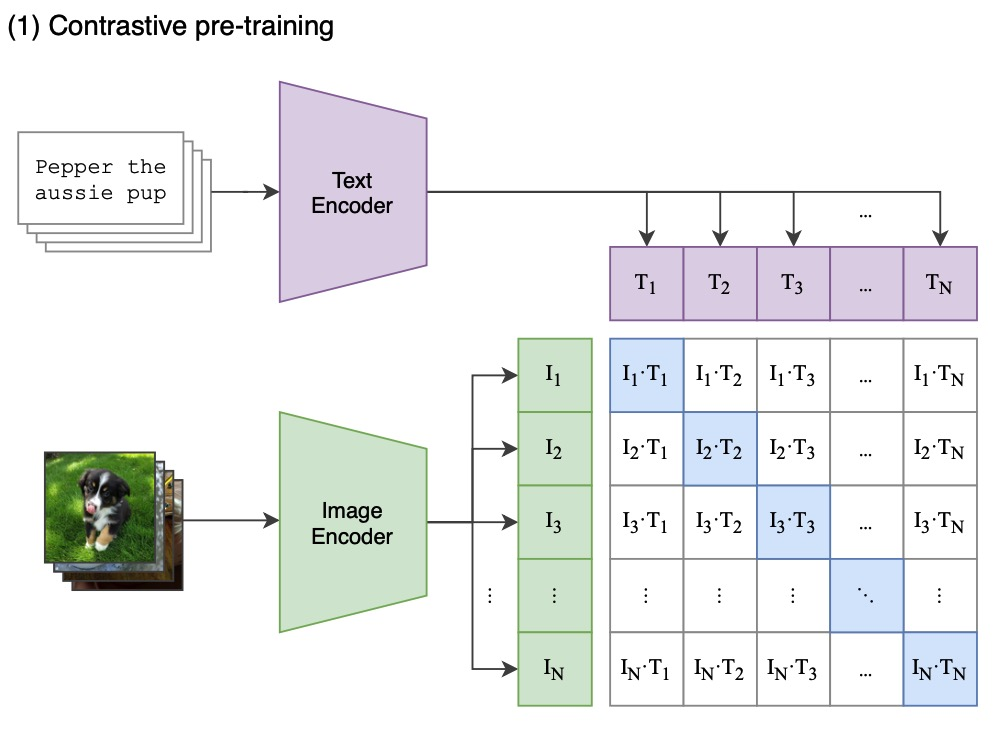
\includegraphics[width=9cm,height=7cm]{p1.jpg}
\caption{CLIP Pretain Pipeline}
\end{figure}

% Please add the following required packages to your document preamble:
% \usepackage[normalem]{ulem}
% \useunder{\uline}{\ul}{}
\begin{table}[]
\begin{tabular}{|l|l|l|}
\hline
Captions                                                                                        & Best room & Worst room \\ \hline
\begin{tabular}[c]{@{}l@{}}The room is pretty big\\  and glorious\end{tabular}               & 1.4899    & 0.2871     \\ \hline
\begin{tabular}[c]{@{}l@{}}The room makes people\\ feel comfortable and relaxed\end{tabular} & 25.326    & 0.5549     \\ \hline
\begin{tabular}[c]{@{}l@{}}The room is well-lighted\\  and drafty\end{tabular}               & 9.4641    & 1.3511     \\ \hline
\begin{tabular}[c]{@{}l@{}}The room is clean and \\ organized\end{tabular}                   & 0.3662    & 0.0304     \\ \hline
\begin{tabular}[c]{@{}l@{}}The room is modern \\ and well-designed\end{tabular}              & 31.511    & 1.2198     \\ \hline
\begin{tabular}[c]{@{}l@{}}The room is small and\\  unexceptional\end{tabular}               & -10.734   & -1.994     \\ \hline
\begin{tabular}[c]{@{}l@{}}The room makes people \\ feel mournful and terrible\end{tabular}  & -1.7917   & -1.413     \\ \hline
\begin{tabular}[c]{@{}l@{}}The room is dark and \\ windowless\end{tabular}                   & -0.5192   & -1.694     \\ \hline
\begin{tabular}[c]{@{}l@{}}The room is disordered \\ and dusty\end{tabular}                  & -1.0322   & -1.356     \\ \hline
\begin{tabular}[c]{@{}l@{}}The room is bare and\\  lifeless\end{tabular}                     & -0.7646   & -3.096     \\ \hline
Final score                                                                                  & 53.3159   & -6.113     \\ \hline
\end{tabular}
\caption{Score of best room picture and worst room picture. The score of a caption shows how related is the picture and the caption. The pictures of rooms are in Figure2.}
\label{tab:my-table1}
\end{table}


Within a batch of size N, the text encoder and image encoder are training to maximize the cosine similarity of N positive pairs of image and text while minimize the cosine similarity of N*N - N negative pairs. The CLIP learns a multi-modal embedding space after pre-training which can be used to find the similarity of an image and a caption. Another contribution is the training data set of CLIP is collected from Internet which is of large scale and noisy. The openAI team publish the paper with several small-scale models, we pick model \textit{"ViT/32"} with best performance to do a downstream task.

The CLIP model is use to score a room picture with five positive comments and five negative comments. We define each positive comment weight 1 and negative comment weight -1.As illustrated in ViLT\cite{ref5}, the CLIP's Modality Interaction part where the relationship of image and text is evaluated is simply so that CLIP may fail to match complex and abstract captions with corresponding images. We propose a simple and effective way of generating comments. The comments consist of two part, \textit{"The room is"} and \textit{a description of room}. The ten comments we chosen are \textit{'The room is pretty big and glorious', 'The room makes people feel comfortable and relaxed', 'The room is well-lighted and drafty', 'The room is clean and organized', 'The room is modern and well-designed', 'The room is small and unexceptional', 'The room makes people feel mournful and terrible', 'The room is dark and windowless.', 'The room is disordered and dusty', 'The room is bare and lifeless'}. We visualize the result by choose room images with the highest mean score and the lowest mean score in Figure2 and Table2.

\begin{figure}[h]
\centering
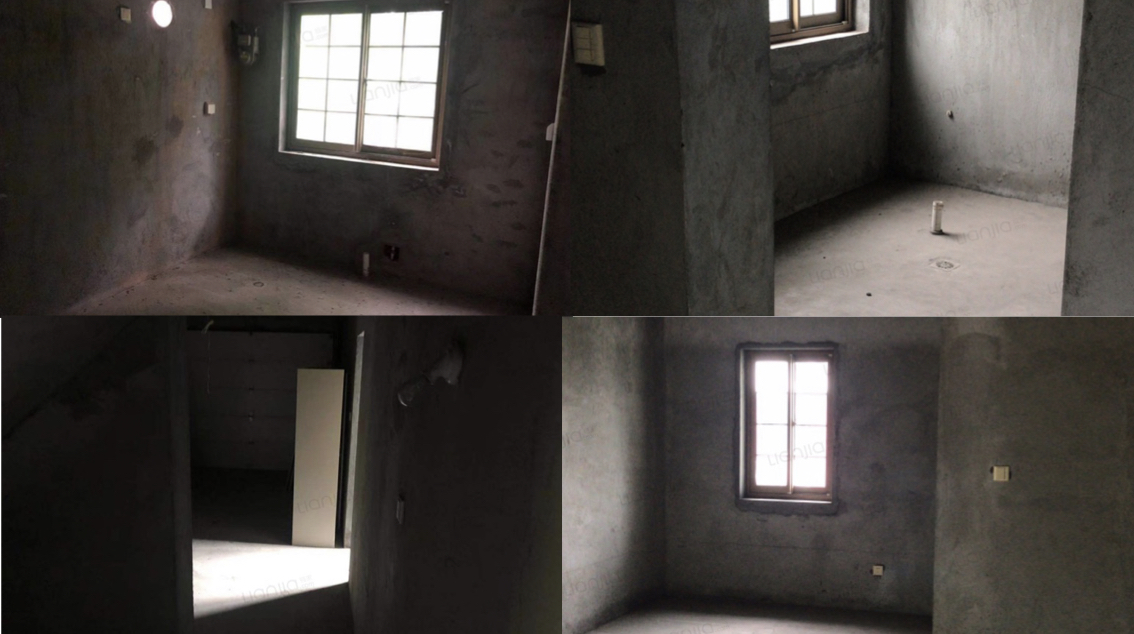
\includegraphics[width=8cm,height=6cm]{p2.jpeg}
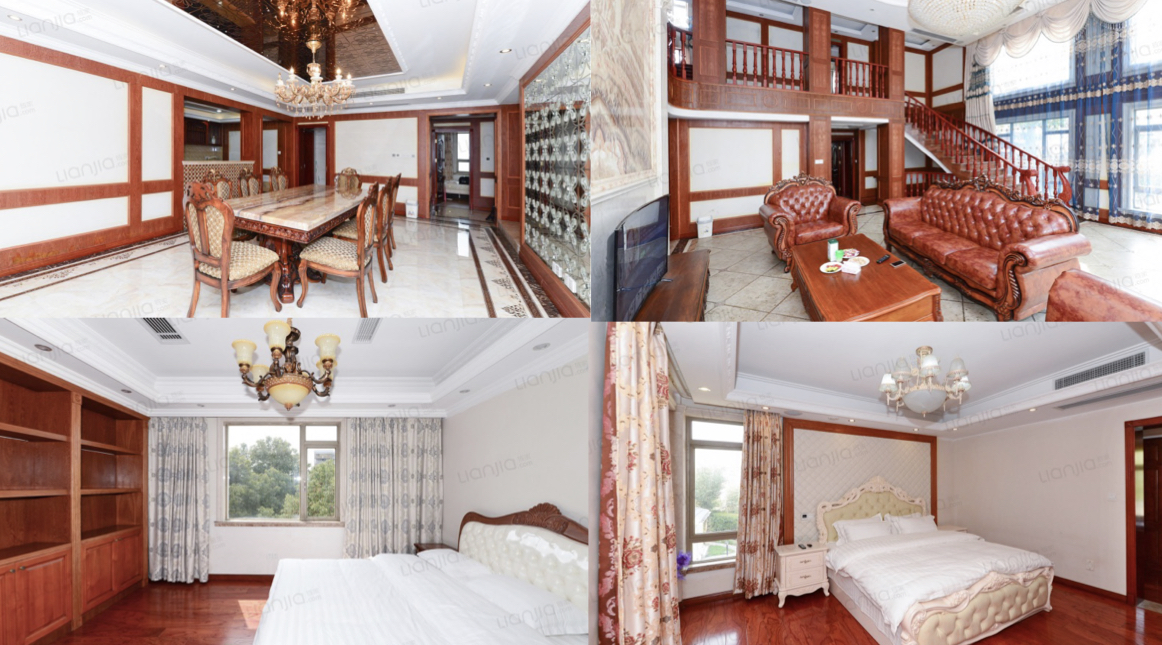
\includegraphics[width=8cm,height=6cm]{p3.jpeg}
\caption{The upper four pictures are the room with lowest score.The lower four pictures are the room with highest score.}
\end{figure}

\subsection{Summary}
The final features contain 58 elements. The detail definition is [house layout(2), house size(1), house detail(16), house facility(10), house description(3), agent(1), house tags(10), geo(2), subway(2), image(10), image number(1)]. The agent feature is the number of houses the agent is currently acting. the subway feature contains the number of subway nearby and the minimum distance to a subway station. The house description feature is a simple measurement of how detail the description is and whether there are hospital or commercial center nearby.
\subsection{Future Work}
There is one idea that have not been implemented. The comments in image embedding may be collect from wiki English corpus by searching key words \textit{"room is"} or other short words describing a room. We may collect large amounts of comments and enlarge the feature vector size of a house. This may leads to better results.

\section{Prediction}
\subsection{Methodology}

\textbf{Regression algorithm}
There are basically two category of regression algorithms, linear regressor and non-linear regressor. Given the feature size is 58, we choose three non-linear regression algorithms, \textit{kernel rigid regression, SVR, decision tree regression}. The kernel rigid regression and SVR need a kernel function to project the input data points into a hyperspace where the data points are more separable than original space.

\textbf{Neural Network}
We propose two architecture of neural network, multiple layer perception and multi-head self attention as Figure3. The MLP architecture consist of one hidden layer, one input layer and one output layer. The multi-head self attention architecture consist of four self attention blocks, where each self attention consist of 10 heads. The self attention architecture was first introduced in Transformer\cite{ref4} and the reason we used it is that self attention layer connects all position with a sequentially executed operations which make it possible for network to capture the relationship between different input features. The multi-head mechanism of self attention layer enables attention layer to capture multiple input features relationship.

\begin{figure}[h]
\centering
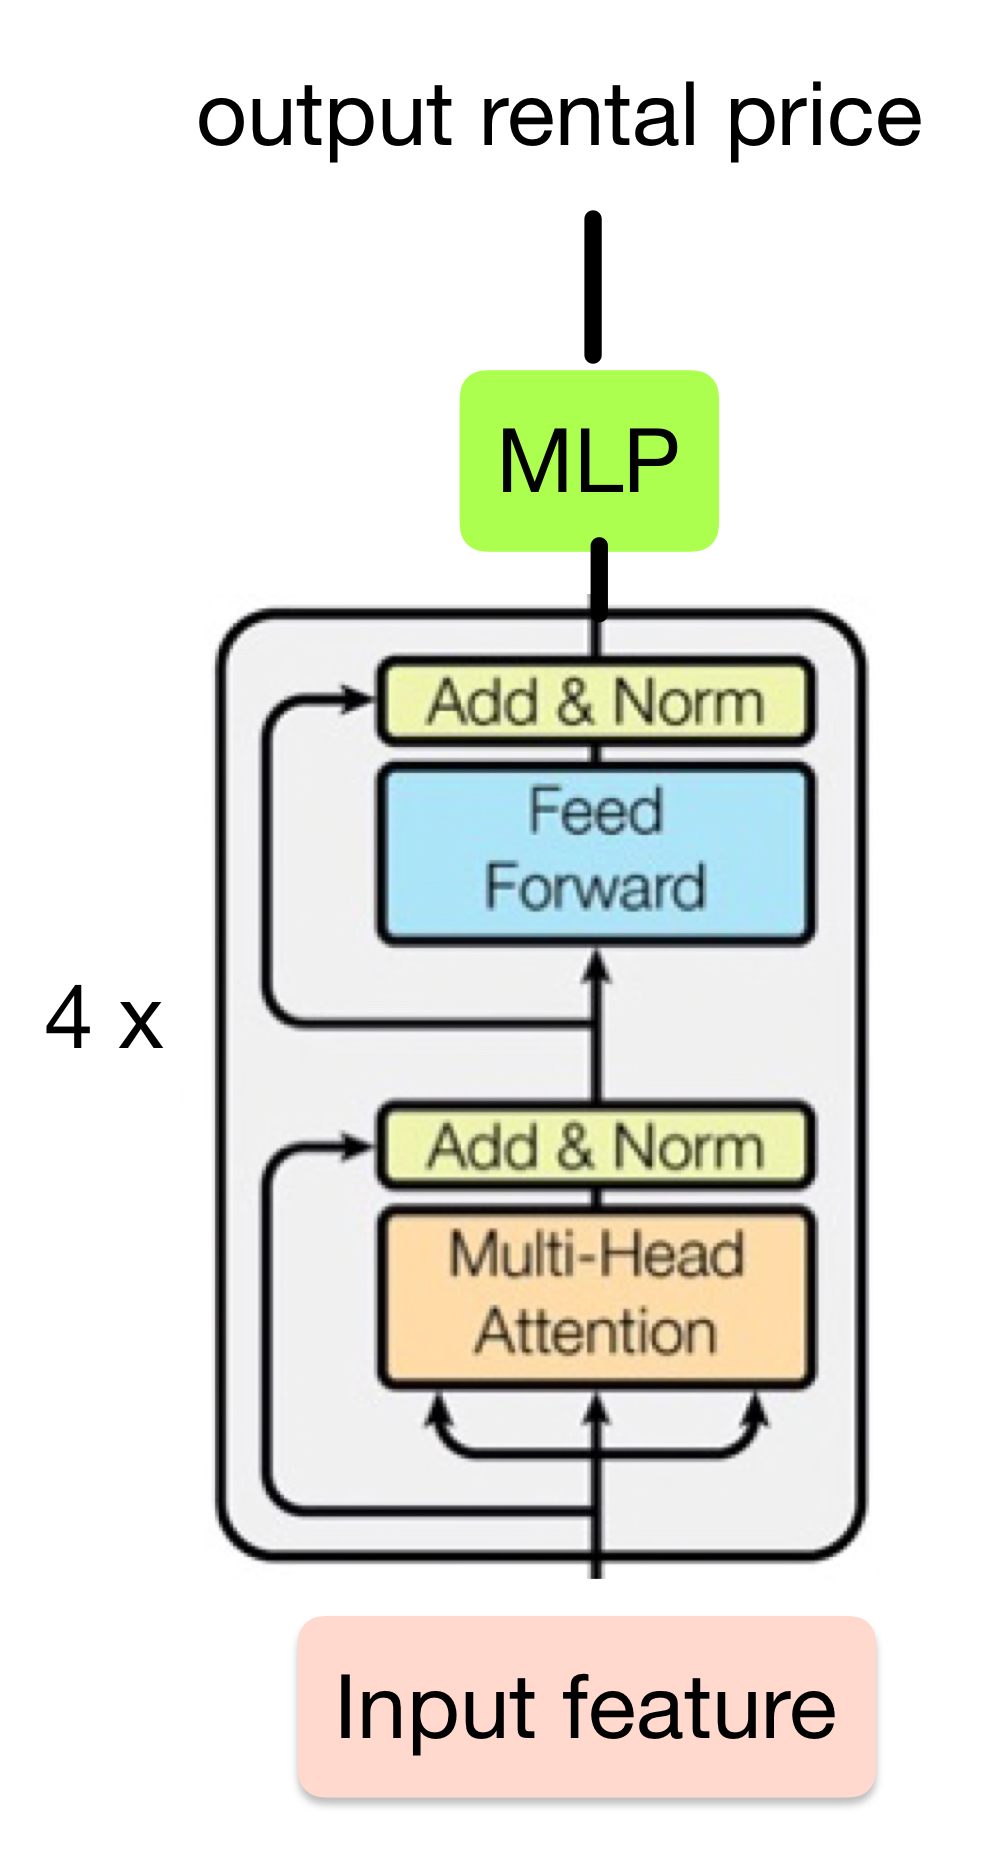
\includegraphics[width=4cm,height=6cm]{p4.jpeg}
\caption{Attention Model Architecture}
\end{figure}

\textbf{Optimizer}
The optimizer we chosen are stochastic gradient descent with weight decay and Adam with weight decay\cite{ref6}. The SGD optimizer is simple but may be problematic when the learning rate or gradients are too large near a local optimum. The Adam alleviate this condition by introducing the first moment estimate and second raw estimate. However, under large scale data set, SGD optimizer may still be a better option for cheaper computational cost than Adam. The optimizer scheduler we choose is cosine annealing and warm restart\cite{ref7}.

\section{Experiments}
\subsection{Experiment Settings}
We spit collected data into 90$\%$ training set and 10$\%$ testing set. Given that the public house rental data won't be noise, the loss function is a modified mean square loss named MMSE for short where the ground truth price is divided by $10^{-4}$. We consider this modification will help us observe the loss value more directly and accelerate convergence speed. Here is the MMSE formula:
\begin{displaymath}
MMSE = \sum_i (pred_i - label_i*10^{-4})^{2}
\end{displaymath}

\subsection{Regression Algorithm}
We test kernel rigid regression, SVR and decision tree regression, for SVR and kernel rigid regression, we test kernel functions \textbf{[linear, polynomial, rbf, laplacian, sigmoid, cosine]}. The result of MMSE loss is in Table5.
\begin{displaymath}
linear: k(x,y) = x^Ty + c
\end{displaymath}
\begin{displaymath}
polynomial: k(x,y) = (\alpha x^Ty + c)^d 
\end{displaymath}
\begin{displaymath}
rbf: k(x_i,x_j) = exp(-\gamma ||x_i - x_j||^2)
\end{displaymath}
\begin{displaymath}
laplacian: k(x,y) = exp(-\frac{||x_i - x_j||}{\sigma})
\end{displaymath}
\begin{displaymath}
sigmoid: k(x,y) = tanh(\alpha x^Ty + c)
\end{displaymath}
\begin{displaymath}
cosine: k(x,y) = \frac{x*y}{||x||*||y||}
\end{displaymath}

\begin{table*}[]
\begin{tabular}{|l|l|l|l|l|l|l|l|}
\hline
                                    & linear   & poly      & rbf       & laplacian & sigmoid  & cosine    \\ \hline
KR with Regularization strength 0.5 & 0.553718 & 2.21813   & 1.275188  & 0.3284159 & 1.440662 & 0.729343  \\ \hline
KR with Regularization strength 1.0 & 0.555052 & 2.21256   & 1.371862  & 0.340766  & 1.440655 & 0.7339337 \\ \hline
KR with Regularization strength 1.5 & 0.555854 & 2.210651  & 1.451493  & 0.3524404 & 1.440649 & 0.731567  \\ \hline
SVR with Regularization 0.5         & 1.177661 &           & 0.7433953 &           & 0.998917 &           \\ \hline
SVR with Regularization 1.0         & 3.206519 &           & 0.69805   &           & 0.877105 &           \\ \hline
SVR with Regularization 1.5         & 9.913045 &           & 0.679994  &           & 0.828925 &           \\ \hline
decision\_tree                      & 1.325817 &           &           &           &          &           \\ \hline
\end{tabular}
\caption{The MMSE of different regression algorithm and different combination of parameters.}
\label{tab:my-table23}
\end{table*}






\subsection{Neural Network}
In all experiment with neural network, we use SGD and Adam optimizer with 0.0001 initial learning rate, 0.00001 weight decay and 0.00001 momentum for SGD. The optimizer scheduler is cosine annealing with warm start where restart begins at 1000iteration. The batch size is 200 and for MLP and Attention architecture, the hidden layer size is 256. We train the 4 combination of model and optimizer for 300 epoch each. The result for MLP is in Figure6,7 and result for Attention is in Figure4,5. The lowest evalution MMSE for Attention network is 73.85 and 42.27 for MLP network. The reason for poor performance is the lack of training data set. We consider data augmentation techniques may alleviate this condition to some extend.

\begin{figure}[htbp]
\centering
\begin{minipage}[t]{0.48\textwidth}
\centering
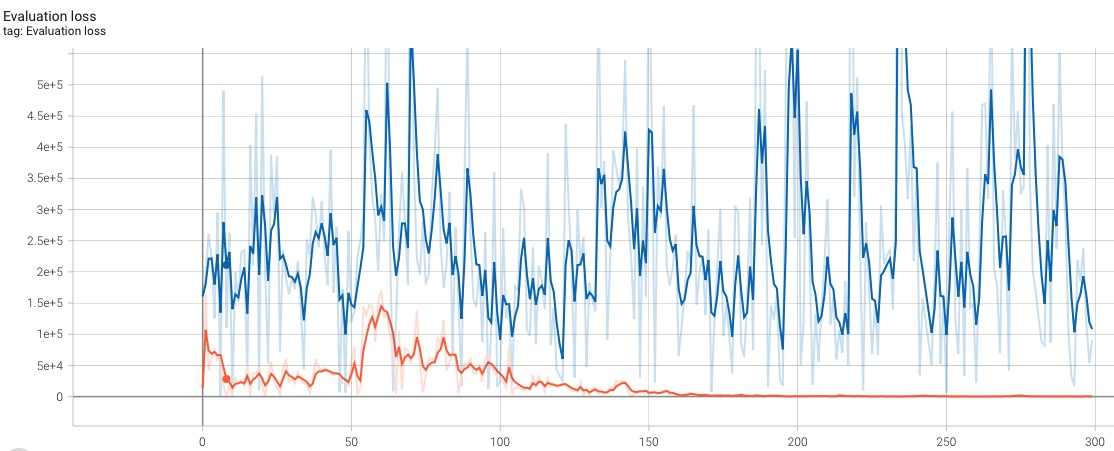
\includegraphics[width=9cm,height=4cm]{Attention Eval.jpg}
\caption{Attention Model Evaluation MMSE Loss. The red line represents the model trained by AdamW optimizer. The blue line represents the model trained by SGDW optimizer}
\end{minipage}
\begin{minipage}[t]{0.48\textwidth}
\centering
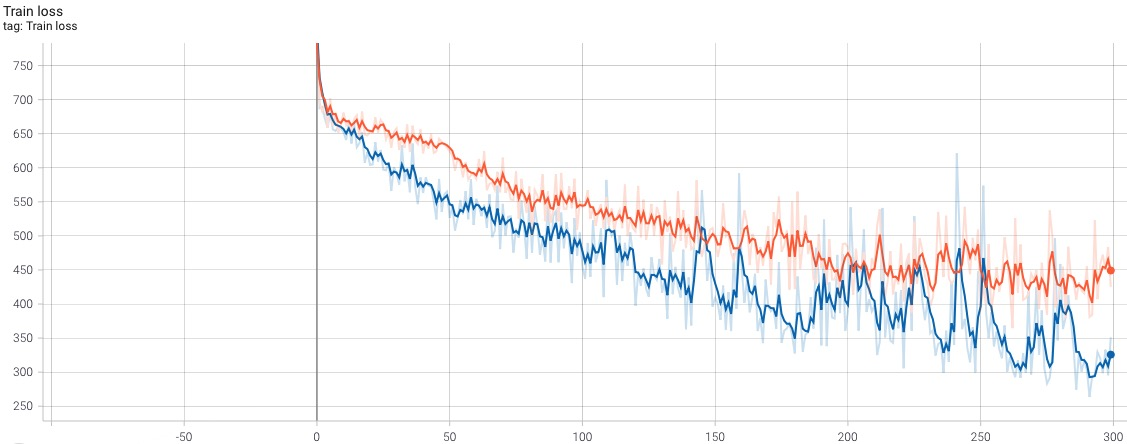
\includegraphics[width=9cm,height=4cm]{Attention train.jpg}
\caption{Attention Model Training MMSE Loss. The red line represents the model trained by AdamW optimizer. The blue line represents the model trained by SGDW optimizer}
\end{minipage}
\end{figure}

\begin{figure}[htbp]
\centering
\begin{minipage}[t]{0.48\textwidth}
\centering
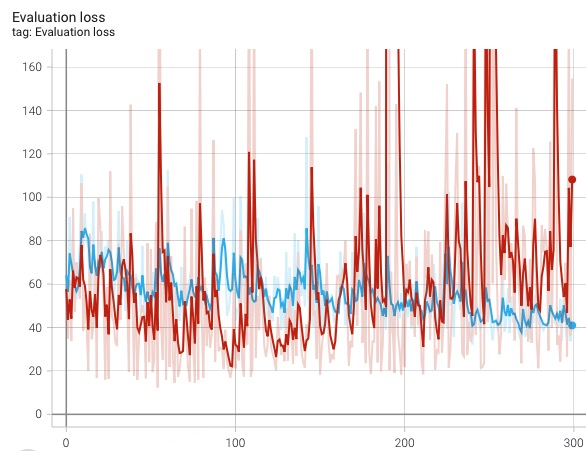
\includegraphics[width=9cm,height=4cm]{MLP eval.jpg} 
\caption{MLP Model Evaluation MMSE Loss. The red line represents the model trained by AdamW optimizer. The blue line represents the model trained by SGDW optimizer}
\end{minipage}
\begin{minipage}[t]{0.48\textwidth}
\centering
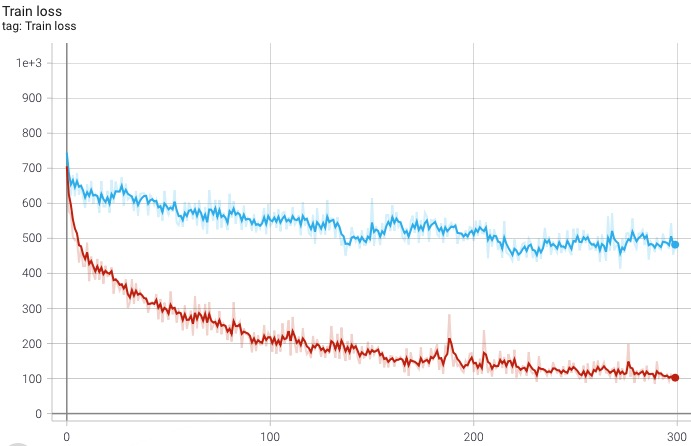
\includegraphics[width=9cm,height=4cm]{MLP train.jpg}
\caption{MLP Model Training MMSE Loss. The red line represents the model trained by AdamW optimizer. The blue line represents the model trained by SGDW optimizer}
\end{minipage}
\end{figure}



% \begin{figure}[h]
% \centering
% 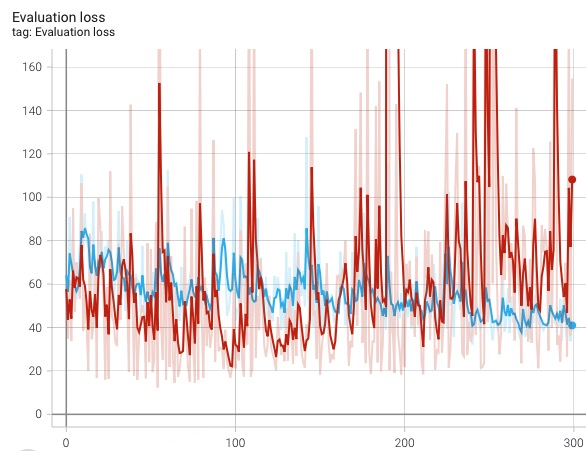
\includegraphics[width=8cm,height=4cm]{MLP eval.jpg} 
% 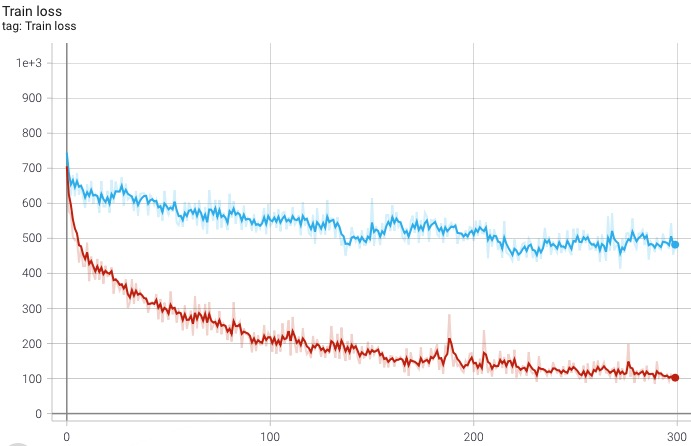
\includegraphics[width=8cm,height=4cm]{MLP train.jpg}
% \caption{MLP Model Loss}
% \end{figure}

\subsection{Feature Analysis}
In this section, we analyze the importance of each feature elements. Here we use the sequential forward selection algorithm. The SFS is a greedy search algorithm which takes the whole feature set as input. The SFS maintains a chosen feature list and will add the element which output highest score when tested with chosen elements. We choose Decision Tree Regressor algorithm as the base testing algorithm. The result of feature importance is in Table6,7. The result show that the most importance feature is the room size. The coordinate of the room is of secondary importance. Intuitively, the room size and the location are the most important factor of rental price and our result demonstrate that. We consider that the latitude and longitude will split the room into different areas, which greatly influence the predicted rental price. Since the coordinate of a room includes the information of nearby subway station, the fact that extracted subway features are of low ranking is reasonable. Surprisingly, we find that the image feature 6, "The room is small and unexceptional" is of third importance. We come to a conclusion that the general negative description of a room will split the rental price in decision tree regressor. 

We also run the experiments with top k features in the rank to see how much features gives best performance. The result is in Table4. The result shows that when we choose top 50 features, the algorithm gives the best performance. The conclusion is that top 50 features are meaningful and will give algorithm useful information while the rest 8 features will confuse the algorithm. However, top 15 and top 35 also give relatively good performance. These two combinations are available options when we are need to find a trade off between model accuracy and computational cost.

\begin{table}[]
\centering
\begin{tabular}{|l|l|}
\hline
Top k & Number of features \\ \hline
5     & 1.7921922284033818 \\ \hline
10    & 1.8748175900326087 \\ \hline
15    & 0.9727805556630434 \\ \hline
20    & 1.7625101513152177 \\ \hline
25    & 1.1438755001195655 \\ \hline
30    & 1.203894725021739  \\ \hline
35    & 0.8164614535326087 \\ \hline
40    & 1.1416450491413044 \\ \hline
45    & 0.743628090673913  \\ \hline
50    & 0.647765078978261  \\ \hline
55    & 0.910040187554348  \\ \hline
58    & 2.0233932191847828 \\ \hline
\end{tabular}
\caption{The MMSE of top k features in decision tree regressor}
\label{tab:my-table21}
\end{table}



\subsection{Ablation Study of Visual Feature}
We investigate how image feature affect our prediction result. We test feature vector with and without image feature by regression algorithms. The result of performance difference is showed in Table3. The positive values in table mean the MMSE loss without image feature is higher than the MMSE loss with image feature. The result shows that the image features plays a positive effect in simple algorithms such as decision tree regressor and kernel rigid regressor with linear, cosine and sigmoid kernel function while image features plays a negative effect in kernel rigid regressor with laplacian, rbf and polynomial kernen function.We think the reason is that in the embedding space of laplacian or polynomial kernel function, the positive and negative image features are not separated, which leads to a drop in performance. From the perspective of feature analysis, we can tell that except for the image feature 6 rank $3^{th}$ in the feature importance, other image features rank behind $30^{th}$. In conclusion, we think the image features do have some positive effects on predicting the rental price, however, the ten descriptions of room pictures should be improved given that some image description features are of low ranking. 




\begin{table*}[]
\begin{tabular}{|l|l|l|l|l|l|l|l|}
\hline
                                    & linear   & poly      & rbf        & laplacian   & sigmoid     & cosine     \\ \hline
KR with Regularization strength 0.5 & 0.0754   & -0.9941   & -0.06648   & -0.0004279  & 4.8E-08     & 0.0004767  \\ \hline
KR with Regularization strength 1.0 & 0.075248 & -0.94053  & -0.07086   & -0.00209    & 5.6E-07     & 0.00030531 \\ \hline
KR with Regularization strength 1.5 & 0.075146 & -0.931651 & -0.073293  & -0.00316424 & 0           & 0.000242   \\ \hline
SVR with Regularization 0.5         & 0.085339 & 0.0002763 & 0.0004     &             & -0.000117   &            \\ \hline
SVR with Regularization 1.0         & 3.20651  & 0.000868  & 0.00058491 &             & 0.000250538 &            \\ \hline
SVR with Regularization 1.5         & -1.2403  & 0.0009    & 0.0007     &             & 9.78E-05    &            \\ \hline
decision\_tree                      & 0.009283 &           &            &             &             &            \\ \hline
\end{tabular}
\caption{The result of ablation experiment. The values are the MMSE of a algorithm without image features minus the same algorithm with image features. If the value is positive, the MMSE of algorithm without image features is higher than the one with image features and images features play a positive effect.}
\label{tab:my-table21}
\end{table*}


% Please add the following required packages to your document preamble:
% \usepackage[normalem]{ulem}
% \useunder{\uline}{\ul}{}
\begin{table}[]
\centering
\begin{tabular}{|l|l|l|}
\hline
Rank & Feature name                  & Description                                                                                \\ \hline
1    & size\_feature                 & The size of room                                                                           \\ \hline
2    & geo\_feature\_1               & Latitude                                                                                   \\ \hline
3    & image\_feature\_6             & \begin{tabular}[c]{@{}l@{}}"The room is small and\\  unexceptional"\end{tabular}             \\ \hline
4    & geo\_feature\_2               & Longitude                                                                                  \\ \hline
5    & tag\_list\_4                  & Well remodelling                                                                           \\ \hline
6    & facility\_info\_feature\_8    & Central heat                                                                               \\ \hline
7    & house\_info\_dict\_park\_no   & \begin{tabular}[c]{@{}l@{}}Whether the parking\\  place is available\end{tabular}          \\ \hline
8    & house\_info\_dict\_west       & The room face west                                                                         \\ \hline
9    & facility\_info\_feature\_4    & \begin{tabular}[c]{@{}l@{}}Whether there is TV \\ in the room\end{tabular}                 \\ \hline
10 & house\_description\_2         & \begin{tabular}[c]{@{}l@{}}Whether a commercial \\ center is mentioned in\\  the description\end{tabular} \\ \hline
11   & tag\_list\_5                  & Newly updated                                                                              \\ \hline
12   & facility\_info\_feature\_1    & \begin{tabular}[c]{@{}l@{}}Whether there is washing \\ machine\end{tabular}                \\ \hline
13   & facility\_info\_feature\_5    & \begin{tabular}[c]{@{}l@{}}Whether there is \\ refrigerator\end{tabular}                   \\ \hline
14   & house\_info\_dict\_east       & The room face east                                                                         \\ \hline
15   & tag\_list\_2                  & Check at anytime                                                                           \\ \hline
16 & house\_info\_dict\_park\_rent & \begin{tabular}[c]{@{}l@{}}Whether there is \\ parking place for rent\end{tabular}                        \\ \hline
17   & house\_info\_dict\_south      & the room face south                                                                        \\ \hline
18   & facility\_info\_feature\_10   & \begin{tabular}[c]{@{}l@{}}Whether there is \\ natural gas\end{tabular}                    \\ \hline
19   & tag\_list\_1                  & \begin{tabular}[c]{@{}l@{}}Strongly recommended \\ house\end{tabular}                      \\ \hline
20   & house\_info\_dict\_heat       & \begin{tabular}[c]{@{}l@{}}Whether there is central\\  heat\end{tabular}                   \\ \hline
21   & house\_info\_dict\_elevator   & Where there is elevator                                                                    \\ \hline
22   & tag\_list\_6                  & Double washrooms                                                                           \\ \hline
23   & house\_info\_dict\_elect      & \begin{tabular}[c]{@{}l@{}}Whether there is \\ commercial electricity\end{tabular}         \\ \hline
24   & house\_info\_dict\_medium     & Medium floor                                                                               \\ \hline
25   & house\_info\_dict\_water      & Commercial water                                                                           \\ \hline
26   & house\_info\_dict\_high       & High floor                                                                                 \\ \hline
27   & house\_info\_dict\_floor      & Exact floor number                                                                         \\ \hline
\end{tabular}
\caption{The rank of feature importance and feature description part1.}
\label{tab:my-table1}
\end{table}

% Please add the following required packages to your document preamble:
% \usepackage[normalem]{ulem}
% \useunder{\uline}{\ul}{}
\begin{table}[]
\centering
\begin{tabular}{|l|l|l|}
\hline
Rank & Feature name                  & Description                                                                                \\ \hline
28   & house\_info\_dict\_checkin    & Checkin at any time                                                                        \\ \hline
29   & layout\_feature\_hall         & Number of halls in room                                                                    \\ \hline
30   & facility\_info\_feature\_3    & Wardrobe                                                                                   \\ \hline
31   & agent\_feature                & \begin{tabular}[c]{@{}l@{}}Number of house a agent \\ is representing\end{tabular}         \\ \hline
32   & layout\_feature\_room         & Number of rooms                                                                            \\ \hline
33   & image\_feature\_9             & \begin{tabular}[c]{@{}l@{}}"The room is disordered \\ and dusty"\end{tabular}                \\ \hline
34   & tag\_list\_9                  & Verified by authority                                                                      \\ \hline
35 & image\_feature\_2             & \begin{tabular}[c]{@{}l@{}}"The room makes people \\ feel comfortable and relaxed"\end{tabular}             \\ \hline
36   & image\_num\_feature           & \begin{tabular}[c]{@{}l@{}}Number of pictures provided \\ by house owner\end{tabular}      \\ \hline
37   & house\_description\_1         & \begin{tabular}[c]{@{}l@{}}Number of section in \\ description\end{tabular}                \\ \hline
38   & tag\_list\_8                  & Pay one deposit one                                                                        \\ \hline
39   & facility\_info\_feature\_6    & hot water heater                                                                           \\ \hline
40   & house\_info\_dict\_park\_free & \begin{tabular}[c]{@{}l@{}}Whether the parking \\ place is free\end{tabular}               \\ \hline
41   & facility\_info\_feature\_9    & Network                                                                                    \\ \hline
42 & house\_description\_3         & \begin{tabular}[c]{@{}l@{}}Whether hospital is\\  mentioned in description\end{tabular}                   \\ \hline
43   & image\_feature\_8             & \begin{tabular}[c]{@{}l@{}}"The room is dark and \\ windowless"\end{tabular}                 \\ \hline
44   & house\_info\_low              & Low floor                                                                                  \\ \hline
45   & tag\_list\_10                 & Monthly rental                                                                             \\ \hline
46   & image\_feature\_5             & \begin{tabular}[c]{@{}l@{}}"The room is modern \\ and well-designed"\end{tabular}            \\ \hline
47   & facility\_info\_feature\_7    & Whether there is bed                                                                       \\ \hline
48   & facility\_info\_feature\_2    & \begin{tabular}[c]{@{}l@{}}Whether there is air \\ conditioner\end{tabular}                \\ \hline
49   & tag\_list\_7                  & near subway station                                                                        \\ \hline
50   & image\_feature\_1             & \begin{tabular}[c]{@{}l@{}}"The room is pretty \\ big and glorious"\end{tabular}             \\ \hline
51   & tag\_list\_3                  & \begin{tabular}[c]{@{}l@{}}Recommended by house\\  owner\end{tabular}                      \\ \hline
52   & image\_feature\_3             & \begin{tabular}[c]{@{}l@{}}"The room is well-lighted \\ and drafty"\end{tabular}             \\ \hline
53   & subway\_feature\_num          & \begin{tabular}[c]{@{}l@{}}Number of nearby subway \\ lines\end{tabular}                   \\ \hline
54   & subway\_feature\_dis          & \begin{tabular}[c]{@{}l@{}}Minimum distance to\\  subway station\end{tabular}              \\ \hline
55   & image\_feature\_10            & "The room is bare and lifeless"                                                              \\ \hline
56   & house\_info\_dict\_north      & The room face north                                                                        \\ \hline
57   & image\_feature\_7             & \begin{tabular}[c]{@{}l@{}}"The room makes people\\ feel mournful and terrible"\end{tabular} \\ \hline
58   & image\_feature\_4             & "The room is clean and organized"                                                            \\ \hline
\end{tabular}
\caption{The rank of feature importance and feature description part2.}
\label{tab:my-table1}
\end{table}

\subsection{Result Analysis}
The result show that given data set size of 9192 and feature vector size of 58. Regression algorithm outperforms neural networks. For regression algorithm, the best model is kernel rigid regression with laplacian kernel function. There are more interesting detail to explore considering different kernel functions have different loss. For neural network, Adam optimizer is more efficient than SGD in training data but leads to a worse evaluation loss in MLP model. However, the Adam optimizer perform better in evaluation loss while the train loss decrease more slowly but more steady than SGD optimizer. The reason may be the convergence speed of Attention model is much slower than MLP model while it can learn more information. However, current data is too little for training both models. Inspired by the success of laplacian kernel function, we believe Graph Neural Network may perform better than MLP and Attention models.

\section{Visualize}
We generate two heat map by \textit{pyechart library} and \textit{baidu map api}. The first heat map is the rental price heat map in shanghai as Figure6. The second heat map is the difference between predicted price and ground truth price as Figure7. For better visualization result, we divided the delta value into several stages.The result of second heat map show that predictions of downtown area are less accurate than other area. The html file of the heat maps are interactive.

\section{Conclusion}
In this project, we investigate the probability of predicting the house rental price from web data. We propose some interesting way of generating feature from raw data. The prediction algorithm are not fine tuned and only used to demonstrate the feasibility of the algorithm. Visualization are made to show directly the trends of data.
\begin{figure}[h]
\centering
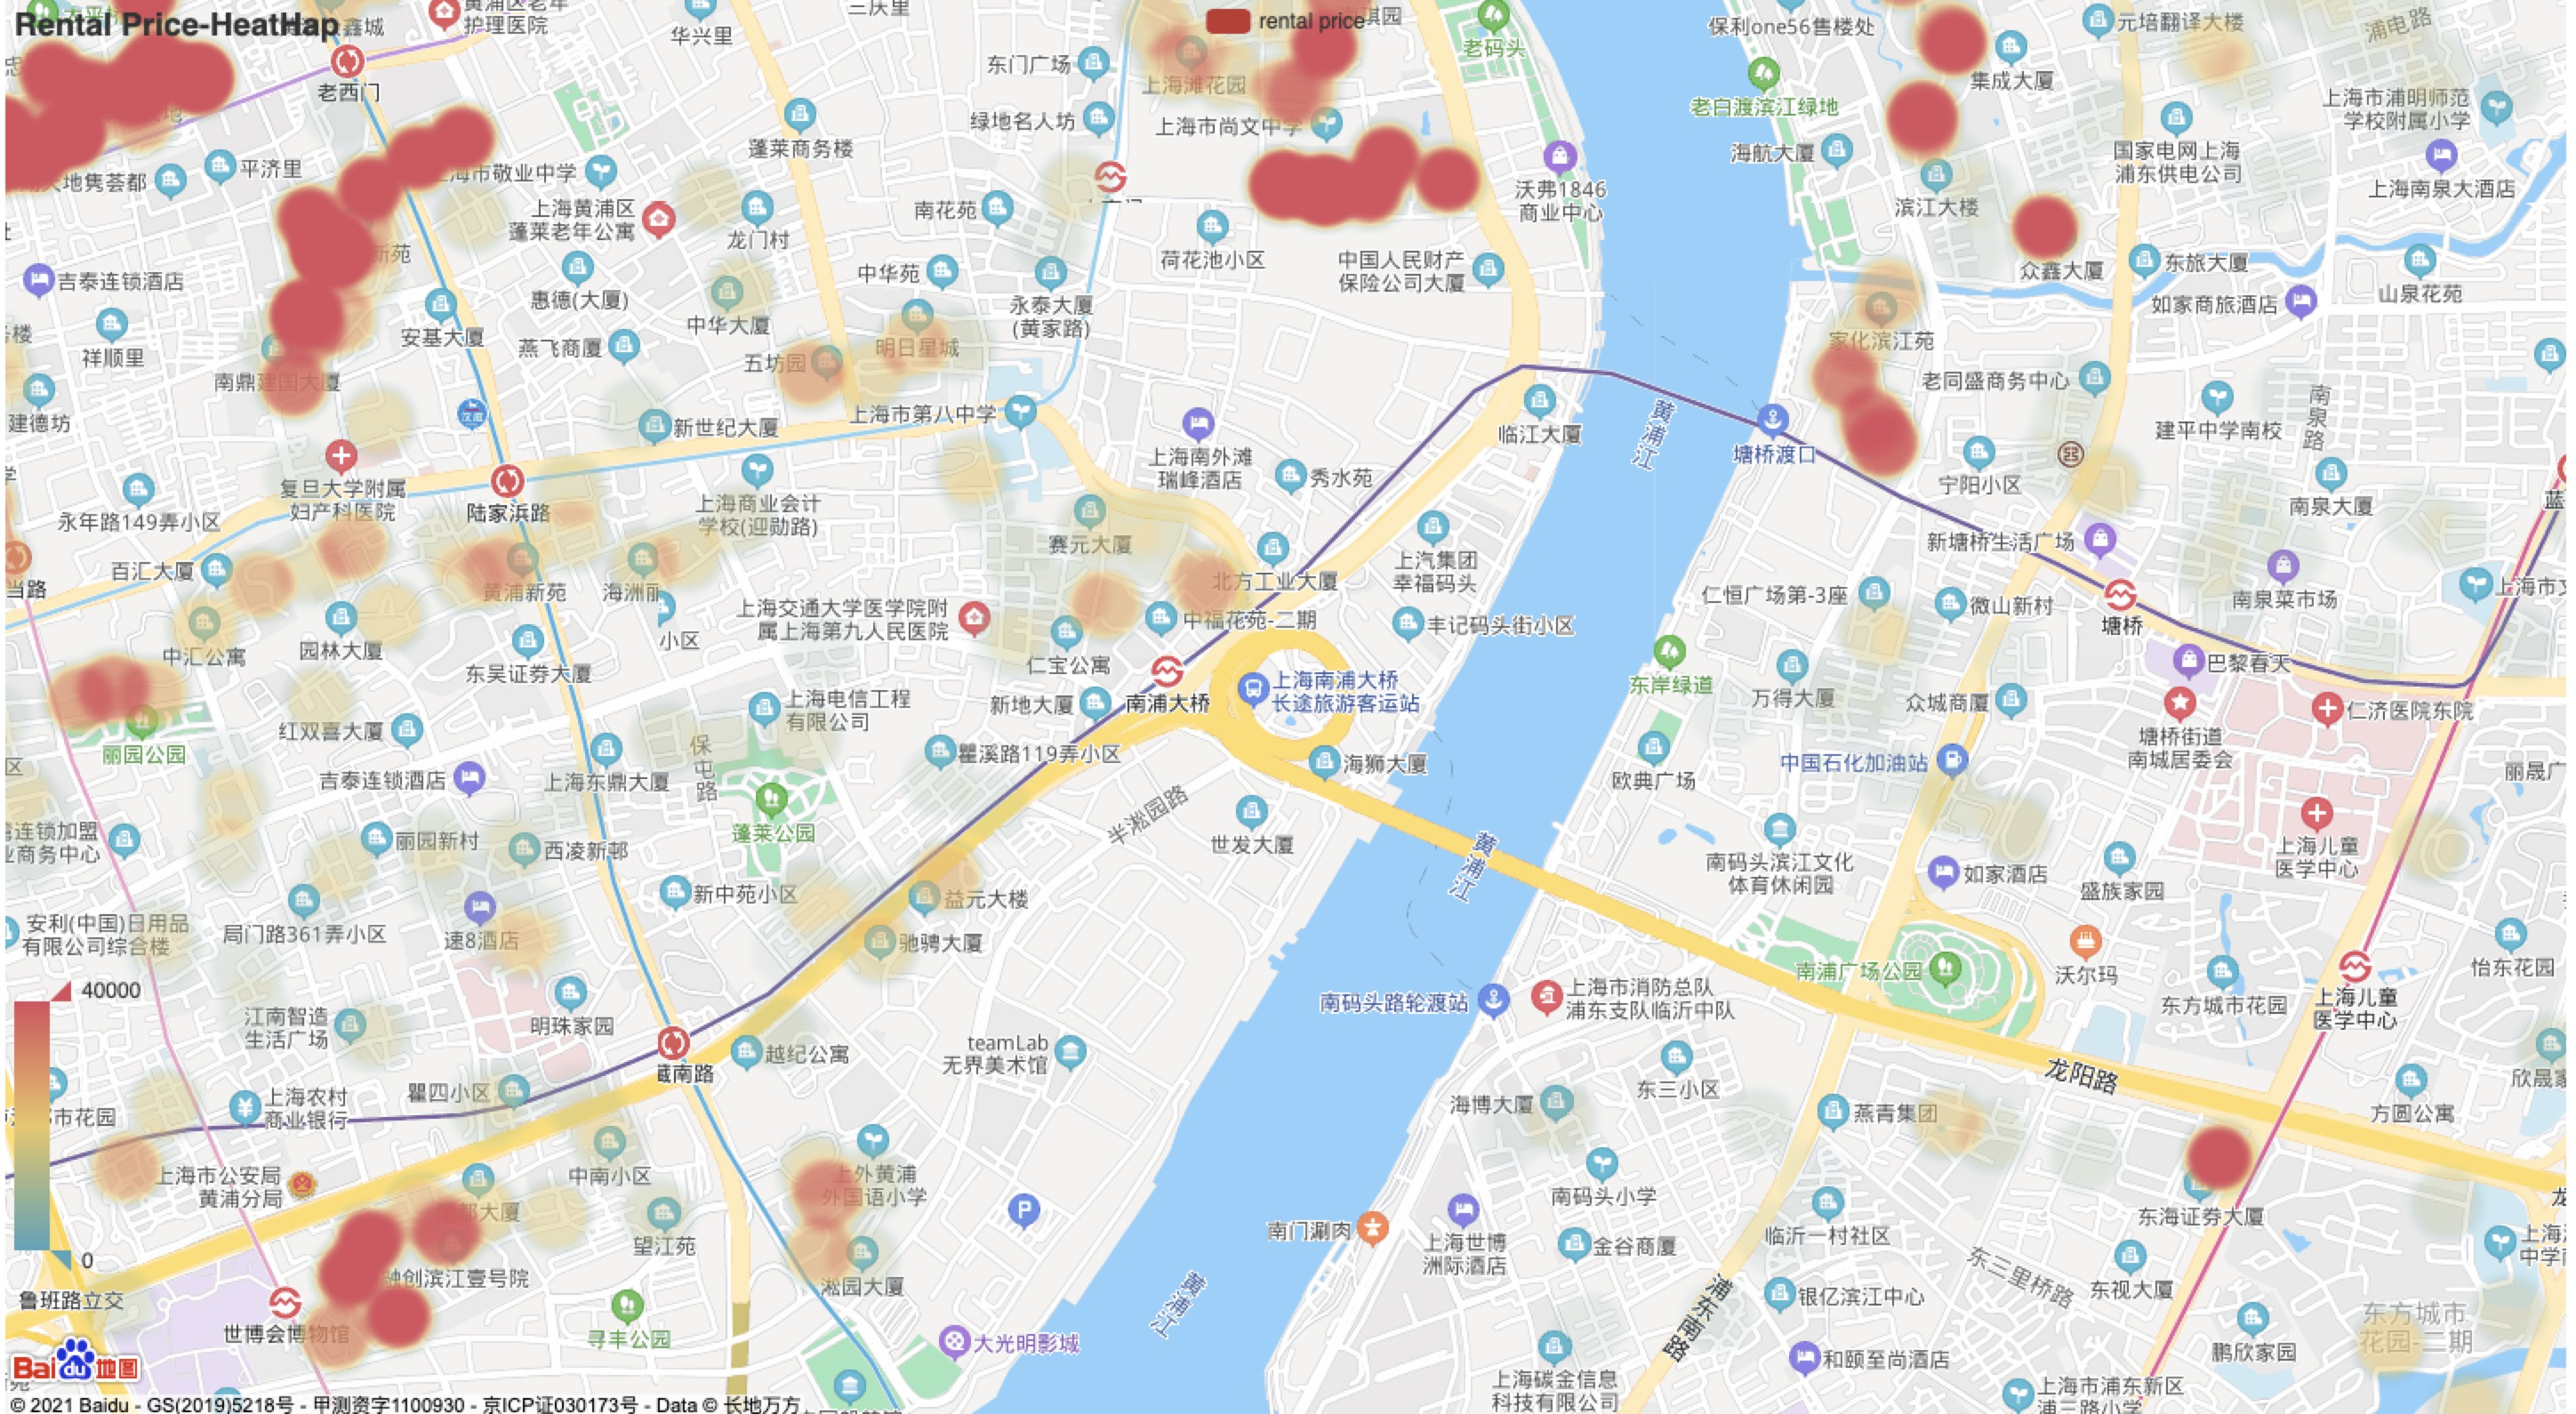
\includegraphics[width=8cm,height=6cm]{p6.jpg}
\caption{Rental Price Heat Map.The darker the red is, the more expensive the rental price is.}
\end{figure}

\begin{figure}[h]
\centering
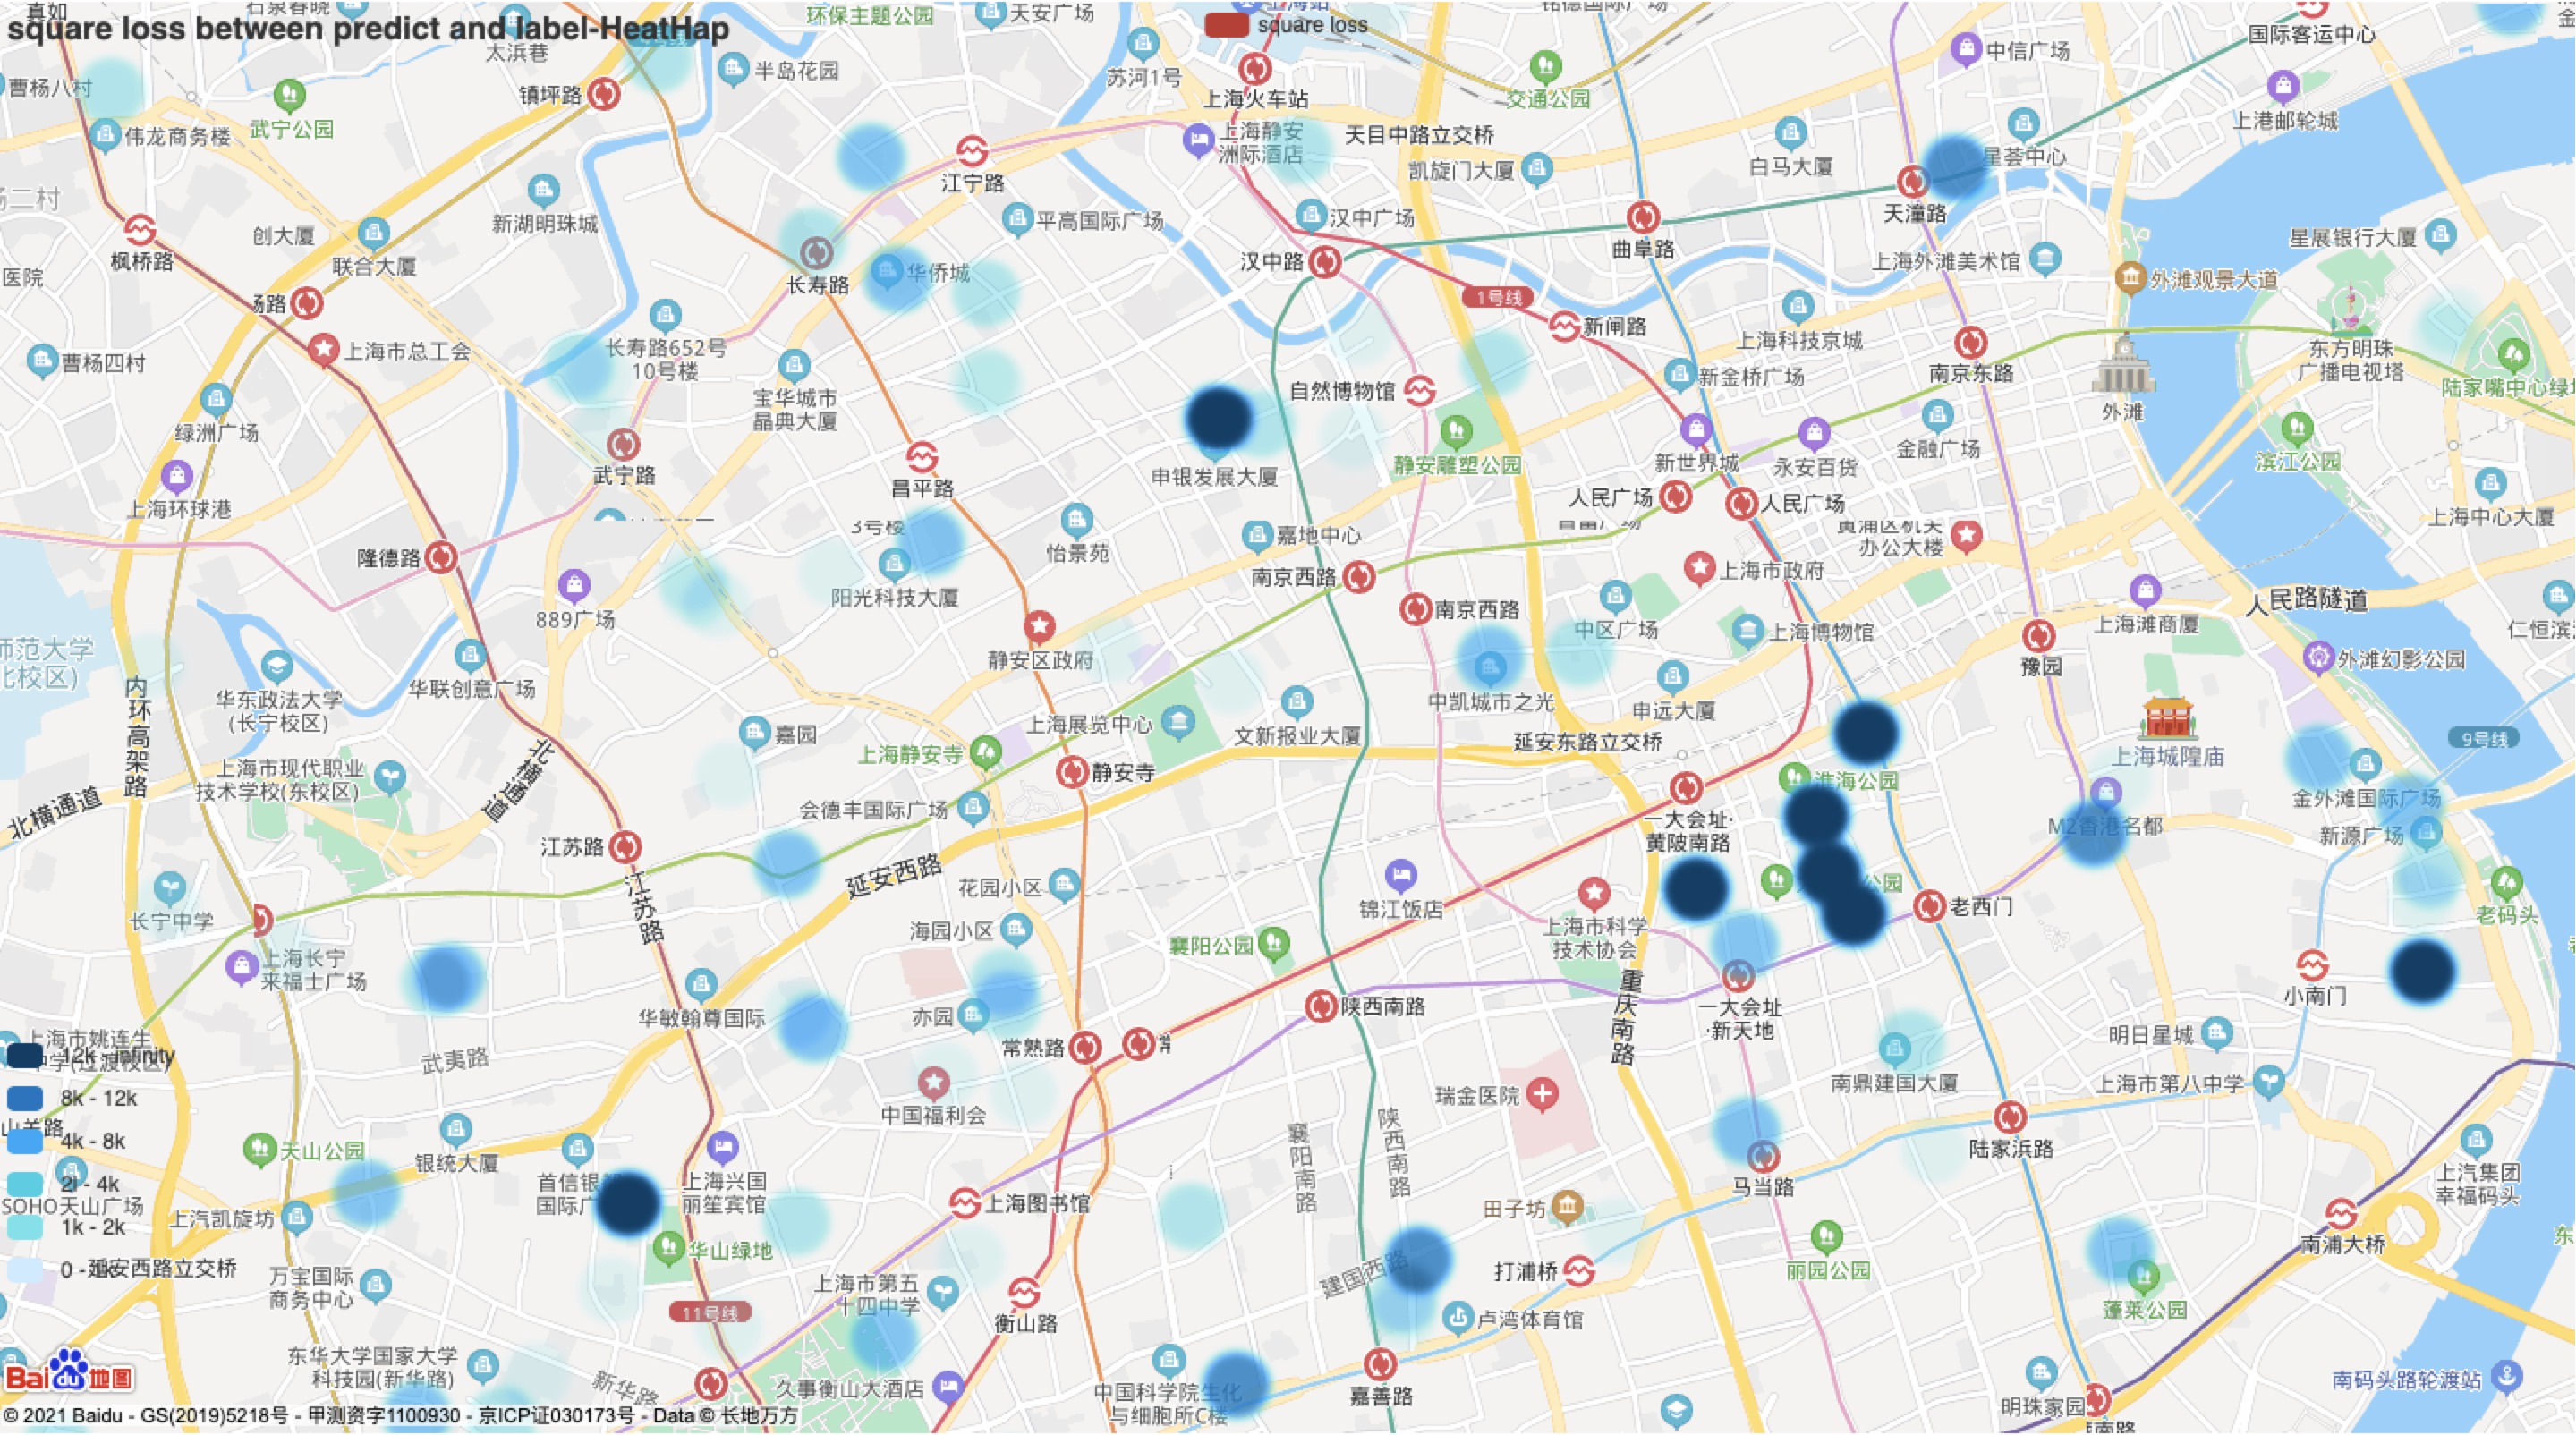
\includegraphics[width=8cm,height=6cm]{p7.jpg}
\caption{Prediction Loss Heat Map.The darker the blue is, the greater the prediction loss is.}
\end{figure}



{\small
\bibliographystyle{ieee_fullname}
\bibliography{egbib}
}


\begin{thebibliography}{99}  
\bibitem{ref1}Radford, A. , et al. "Learning Transferable Visual Models From Natural Language Supervision." (2021).
\bibitem{ref2}Dosovitskiy, A. , et al. "An Image is Worth 16x16 Words: Transformers for Image Recognition at Scale." (2020).
\bibitem{ref3}He, K., Zhang, X., Ren, S., and Sun, J., “Deep Residual Learning for Image Recognition”(2015).
\bibitem{ref4}Vaswani, Ashish, et al. "Attention is all you need." Advances in neural information processing systems. 2017.
\bibitem{ref5}Kim, Wonjae, Bokyung Son, and Ildoo Kim. "Vilt: Vision-and-language transformer without convolution or region supervision." arXiv preprint arXiv:2102.03334 (2021).
\bibitem{ref6}Loshchilov, Ilya, and Frank Hutter. "Decoupled weight decay regularization." arXiv preprint arXiv:1711.05101 (2017).

\bibitem{ref7}Loshchilov, Ilya, and Frank Hutter. "Sgdr: Stochastic gradient descent with warm restarts." arXiv preprint arXiv:1608.03983 (2016).

\end{thebibliography}

\end{document}



